%\documentclass[11pt]{amsart}
\documentclass[11pt]{scrartcl}
\usepackage[top=1.0in, bottom=1.0in, left=1.0in, right=1.0in]{geometry}
\geometry{letterpaper}
\usepackage{graphicx}
\usepackage{amssymb}
\usepackage{epstopdf}
\usepackage{listings}
\usepackage{color}
\usepackage{booktabs}
\DeclareGraphicsRule{.tif}{png}{.png}{`convert #1 `dirname #1`/`basename #1 .tif`.png}
\title{Similar Days at Airports in the New York Area}
\author{Akhil Shah, Kenneth Kuhn, Chris Skeels}
%\date{}
\begin{document}
\maketitle


\section*{Executive Summary}
This report describes our investigation of various methodologies for clustering calendar days using data summarizing forecast and observed weather and air traffic at key airport in the New York area.  We are primarily interested in identifying sets of similar days where similarity is defined in terms of the conditions that lead to the implementation of various Air Traffic Flow Management Initiatives (ATFMIs) such as Ground Delay Programs (GDPs).  The work here represents a first step toward the construction of a decision support tool for dispatchers at airline operations centers and officials at the Federal Aviation Administration's Air Traffic Control System Command Center (ATCSCC) that plan ATFMIs.  Our secondary interest is in surveying reasonable approaches for clustering calendar days in aviation systems research.  We describe the identification of similar days using the following sequence of steps: collecting available data sets, defining features within the data, clustering using various Machine Learning algorithms, and assessing the obtained results.

Terminal Area / Aerodrome Forecast (TAF), Aviation Routine Weather Report (METAR), and Localized Aviation MOS (Model Output Statistics) Product (LAMP) data are all useful data sets for describing airport weather.  TAF and LAMP data describe forecast conditions while METAR data describe observed conditions.  Historical archives of all three types of data exist, although coverage and availability are often limited when it comes to TAF data.  Aviation System Performance Metrics (ASPM) data summarize scheduled and observed airport operations.  ATFMI advisory data can be analyzed to see when and where ATFMIs have been implemented.

Table 1 details examples of reasonable methodologies for clustering calendar days for aviation systems research.

\begin{table}[htdp]
\caption{Reasonable Approaches for Clustering Days by Conditions at Airports}
\begin{center}
\begin{tabular}{|l|l|l|l|}
\hline
{\bf Data Sets}&{\bf Feature Selection}&{\bf Labels Applied}&{\bf Clustering}\\
&{\bf Methodology}&&{\bf Algorithm}\\
\hline 
TAF data, & Knowledge based &Presence/Absence& k-means\\
ASPM data,&& of GDPs&\\
ATFMI advisory data&&&\\
\hline
Traffic Biasing & K-means\\
\hline
Temporal PCA & K-means\\
\hline
Traffic Biasing & DBSCAN\\
\hline
\end{tabular}
\end{center}
\label{default}
\end{table}%

\section*{Introduction and Context}
Personnel at the Federal Aviation Administration's Air Traffic Control System Command Center and at airline operations centers regularly implement Air Traffic Flow Management Initiatives (ATFMIs) purposefully delaying, canceling, and rerouting flights. These initiatives increase the safety and efficiency of the nation�s air transportation system, for example by replacing airborne delay with ground delay, and are necessary during inclement weather and in other situations where demand for system resources exceeds capacity.  In particular, problems at airports often create the need for ATFMIs.  Analysis of the past use of ATFMIs can demonstrate the relative success of courses of action but must account for the distinct conditions faced during planning and operations.  An identification of days that are similar can help, for example allowing analysts to focus on the 10 days in the past two years when there was thunderstorm activity at the key airports in the New York area between 8am and 11am, local time, but clear weather the rest of the day.

This report describes our work to develop methodologies for the identification similar days in terms of aviation weather and air traffic operations at the airports in the New York area.  This report follows an earlier report to identify similar days based on conditions in the airspace around New York City.  We do not wish to replicate the prior report and thus only report on new findings specific to our study of airports.  The earlier report includes more detail regarding why it would be beneficial to identify similar days from the perspective of ATFMI planning or operations.

As in our earlier work that focused on the airspace, we have published many of our results focusing on airports in a web based application.  The application is a minor update of the version we developed and reported on previously.  The earlier report contains a more complete description of our web based application, and we here only highlight recent changes.

In this report, we primarily report on our work to identify features that describe aviation weather and air traffic at airports in the New York area, the data sets we use to define these features, and interesting results we obtain.  The final section of this report is a conclusion that compares the airport-focused results to the airspace-focused results obtained previously.

\section*{Airport Weather and Air Traffic Data}
We are interested in describing forecast and observed aviation weather and air traffic at airports in the New York area.  We focus on John F.\ Kennedy International Airport (JFK), Newark Liberty International Airport (EWR), and LaGuardia Airport (LGA).  These are the busiest airport in the region, by some distance.  Our methods could be applied to other airports in the area, or in other areas, relatively easily.

Airports themselves issue Terminal Area/Aerodrome Forecast reports (TAFs) and Aviation Routine Weather Reports (METARs) which summarize local weather conditions. METARs can contain select forecast data but, generally speaking, TAF data are forecast data while METAR data are observational data. TAF and METAR data contain information on: wind speed and direction, wind gusts, visibility, precipitation, cloud height, cloud cover, humidity, and pressure. Prior research efforts have linked many of these variables to traffic flow management initiatives. Previous studies \cite{smith2009decision} have  successfully used TAF data to forecast Ground Delay Program initiation, but without giving details on the relative importance of specific variables.  The authors in \cite{mukherjeepredicting} point out the relevance of hourly observations of visibility, cloud height, wind, convection, and precipitation in particular, again for predicting GDPs. TAFs and METARs are issued roughly hourly to ensure reports keep up with changing weather conditions but also that distinct consumers of the data have a consistent report and time to plan against it.  A related study \cite{wolfe2011method} analyzed combinations of features (``queries") from airport-specific Weather Impacted Traffic Index (WITI) data to determine which were most relevant in predicting observed weather-related GDP from present time to six hours in the future.  They developed an information-retrieval model consisting of thresholding WITI features as queries or rules.  Their model was trained using observed 2008 GDP data, as recorded in the National Traffic Management Log (NTML), and tested on 2009 GDP data.  However this study concluded that the rules based on WITI features were only slightly more predictive than a constant rule which always predicted ``no GDP'. 

A collection of hourly observations of TAF and METAR data, or other data detailing the variables included in TAF and METAR data, covering the busiest airports in the New York area over an extended period of time would comprise an ideal data set to describe airport weather in the area at the time.  Current TAF and current METAR data are available. A large volume of METAR data has been collected in a publicly accessible historical archive. While there are repositories of TAF data, such as www.ogimet.com and the NASA Data Warehouse, none have the same coverage and availability as the repository of METAR data. This result is unsurprising; there are relatively many uses for historical observations of weather conditions and relatively few for historical forecasts. Luckily, there is an alternate data source that does contain both forecast and observed weather at airports. The National Oceanic and Atmospheric Administration's (NOAAs) Localized Aviation MOS (Model Output Statistics) Product (LAMP) combines much of the same data that appears in TAF and METAR data. This data is free to download from NOAA. Table 2 summarizes the availability of useful airport weather data.

Traffic flow management is concerned with mitigating temporary supply and demand imbalances. At the level of an airport, the primary concern is almost always that the number of aircraft scheduled to land at and take off across a set block of time may be higher than the throughput of the runways will allow. A reasonable length for such a block of time would be an hour or a few hours. Supply-demand imbalances over shorter periods of time, e.g., two aircraft scheduled to land at the same time, can be accommodated with minor path adjustments rather than the more strategic traffic flow management initiatives. Hourly observations of scheduled operations could be easily compared to weather data such as TAFs and METARs that are reported hourly. A collection of hourly observations of the numbers of aircraft scheduled to land at and take off from the busiest airports in the New York area would be an ideal data set here.

\begin{table}[htdp]
\caption{Summary of Airport Data}
\begin{center}
\begin{tabular}{|c|c|c|}
Name & Feature & Notes
\end{tabular}
\end{center}
\label{default}
\end{table}

\subsection*{LAMP Data details}
An overview of LAMP can be found in \cite{ghirardelli2005overview}.  LAMP data is produced roughly hourly and and covers airports in the continental United States, Hawaii, Alaska and Puerto Rico.  For data sources it uses both surface observations and radar data.  The main premise of LAMP is that the most recent surface observations (mostly METAR reports, used as reported after undergoing quality control checks) can have strong predictive value in updating MOS. Radar data (16-level 2km WSI and 7-level 10km RCM) used as predictors for thunderstorm development.  Observed lightning from National Lightning Detection Network used in development of thunderstorm probabilities. 

The following are forecasted by LAMP:
\begin{itemize}
\item{Prob. of precipitation $>$ 0.01 inches in 6 or 12h period}
\item{Precipitation type (liquid, snow, freezing) conditional on precipitation occurring}
\item{Probability of ceiling height belonging to a fixed set of altitudes}
\item{Probability of total sky cover belonging to a fixed set of categories (e.g. clear, few, overcast, etc.)}
\item{Probability of visibility belonging to a fixed set of ranges}
\item{Probability of obstruction to vision belonging to a fixed set of categories (e.g. haze, mist, fog, etc.)}
\item{Probability of thunderstorm in 2h bins (for 25h out since start of LAMP run)}
\end{itemize}

\subsection*{METAR data details}
METAR variables include: temperature, dew point, humidity, sea-level pressure, visibility, wind direction, wind speed, gust speed, precipitation, condition code, event code.

\section*{Selecting Features to Describe Airport Conditions}
It is important to note that the dominant factor which determines the quality of any machine learning (or more generally, statistical model) approach is the selection of features that are most relevant rather than the choice of prediction or clustering algorithms.  Generally, the best source for relevant features are derived from expert domain knowledge.  However machine learning methods for automated feature selection can complement such expert elicitation by quantifying the relevance of each feature.  Moreover feature selection methods usually rely on having a dataset with accompanying ground truth labels.  For example, if we were interested in determining which weather and traffic features were most relevant to predicting a Ground Delay Program (GDP) on any given day, the feature selection algorithm would require a ``training" dataset that included not only the predictors (weather and traffic) but also the observed ground-truth label of absence or presence of GDP for each data record \cite{mukherjeepredicting}.  The goals of this algorithm would be to model current GDP decision making and/or to forecast future GDP decisions.  Our primary goal was somewhat different, to explore, characterize, and categorize airport weather and traffic conditions without modeling current GDP decision making.  Therefore, it was not appropriate, for our study, to use ground-truth labels.  The lack of ground-truth labels rules out various feature selection methods \cite{guyon2003introduction}.  Methods for feature selection and cluster analysis in an `unsupervised' environment like ours are often based on finding the most clearly defined clusters possible.  While we are interested in finding clearly defined clusters, where possible, we are most interested in identifying features that summarize and characterize how analysts and air traffic control planners describe airport weather and air traffic at airports\dots

Our clustering results were derived from features that were selected by either surveying the literature for those considered relevant or using heuristics.  In the sections below we summarize the literature employed for knowledge-based feature selection and also our heuristic methodologies: Traffic Biasing and Temporal PCA.
\subsection*{Knowledge-Based Feature Selection}
Previous studies have employed airport-centric observations and forecasts of weather and traffic data for clustering days.  We will use these weather and traffic features identified as relevant as part of our overall clustering analysis.  In these studies, features are initially identified based on domain knowledge, and then filtered for relevancy using either correlation analysis or other statistical measures, when used as explanatory varaibles in a statistical model for predicting the observed TFM data \cite{mukherjeepredicting,grabbe2013similar}.  

In \cite{mukherjeepredicting}, the authors employ logistic regression and decision trees to predict the absence or presence of GDP every hour at EWR.  Explanatory variables which are determined as statistically significant as predictors include:
\begin{itemize}
\item{the present hours visibility,}
\item{the demand-to-capacity ratio and queueing delay as derived from hourly scheduled arrival data and the assumed arrival capacity,}
\item{the wind speed,}
\item{the Weather Impacted Traffic Index for the local Air Route Traffic Control Center (ZNY - New York Center),}
\item{and the averages, over the preceding three hours, of the wind speed, demand-to-capacity ratio, and ZNY WITI.}
\end{itemize}
These seven features were determined to be statistically significant as predictors of hourly GDP at EWR, whereas cloud ceiling and cross-winds at EWR were deemed to be not.  

In \cite{grabbe2013similar} the authors performed clustering of EWR airport-level data which included observed hourly arrivals and hourly wind speed, wind gusts, wind direction, and ceiling.  These features were selected as relevant by performing a correlation analysis with the absence or presence of hourly GDP at EWR.  Note unlike the previous analysis, visibility at EWR was determined to be not as strong a predictor of GDP, and thus was not used in subsequent clustering\footnote{Textural descriptions of precipitation were also presumably ruled out as relevant and thus not employed in their clustering analysis.}

As an alternative to generating clusters of days, the authors of \cite{liu2014} employ a semi-supervised  method to identify similar days to a given day using a distance metric applied to hourly forecasted weather data on those days at a given airport (using TAF data).  One of their main contributions is to derive a distance metric from user supplied specifications of sets of similar and dissimilar hours.  The authors suggest and apply a specific method for finding similar and dissimilar hours based on runway configuration, Airport Acceptance Rates (AAR), and whether visual or instrument meteorological conditions are in effect.  The derived (learned from data and user supplied specifications) distance metric minimizes the distance between weather feature vectors at hours that are defined to be similar, while ensuring the distance between feature vectors at dissimilar hours is greater than one. Employing such a semi-supervised distance metric, their proof-of-concept example selects two days in 2012 at EWR and using a distance metrics, learned from similar and dissimilar hourly specifications for 2011 TAF and ASPM data, derives the five most similar days from 2011 to each of the two given 2012 days.  Their feature vector is nine-dimensional and consists of boolean values for absence/presence of thunderstorm and snow, and various functional transformations of visibility, ceiling and wind speed.

Based on the literature, we define features that include, for each day, three-hour averages for each of the following variables: scheduled arrivals, scheduled departures, visibility, and wind speed.
 
\subsection*{Traffic Biasing}
Both our weather and traffic datasets contain hourly observations of many variables. Attempting to use all observations as features would produce a data set that is too large for most clustering algorithms, owing to the curse of dimensionality.  A na{\"i}ve mitigation strategy would be to uniformly average the values of numerical variables over a set of 24 hourly observations to produce a single value for a given day.  This would, however, treat all observations as equally important when we are interested in weather as it relates to air traffic and we know that air traffic is busier at certain times of day.  A more sophisticated approach would be to employ a weighted average approach where weights are determined through the following heuristic: determine daily average arrival count for a given airport, and normalize these counts to sum to one.  In our case we used ASPM scheduled arrival and departure counts from 2010-2013 to determine the average hourly arrival for each of the three New York region airports in our analysis.  Once normalized, these form 24 weights $w_h$, where $h$ is the hour index, and are then used to form the weighted average for the METAR numerical variables.  For example, a given day's visibility at JFK would have the following expression to reduce the 24 observed values to a single value $v^{TB}_{d} = \sum_{h}^{24} w_h v_{dh}$, where $d$ is the index for a given day in the dataset.  We call this approach traffic biasing.

Below we show the hourly variation of arrival data at JFK for every day between 2010-2013.  Note that there is a clear pattern; some hours are much busier than others.  The traffic biasing heuristic uses this information, weighting weather observations more when they were recorded at a time when there was more air traffic scheduled to use the airport.

\emph{insert box plot of hourly arrivals at JFK here}


\subsection*{Temporal PCA}
Another heuristic we have explored for feature selection is based on Principal Component Analysis (PCA) and, similar to traffic biasing, converts hourly observations of a variable to a daily summary statistic.  PCA is used to select the linear combination of the 24 observed values of each variable per day which captures the largest possible variation between days (i.e. the first PCA component).  Our earlier airspace-focused report describes how PCA can be used to automatically select features for a subsequent cluster analysis.

Below we show the first three PCA components of a given day at JFK for various weather variables recorded in METAR data.  Note that some variables do have strongly explanatory first PCA component, but others do not.

\emph{insert box plot of hourly arrivals at JFK here}

\section*{Results and Discussion}
\subsection*{Exploratory Analysis}
Below we summarize the statistical variation of the datasets we have used to derive features and cluster days.  

Variation over 24 hours of selected METAR weather variables for days in 2010-2013.

\begin{figure}[htbp]
\begin{center}
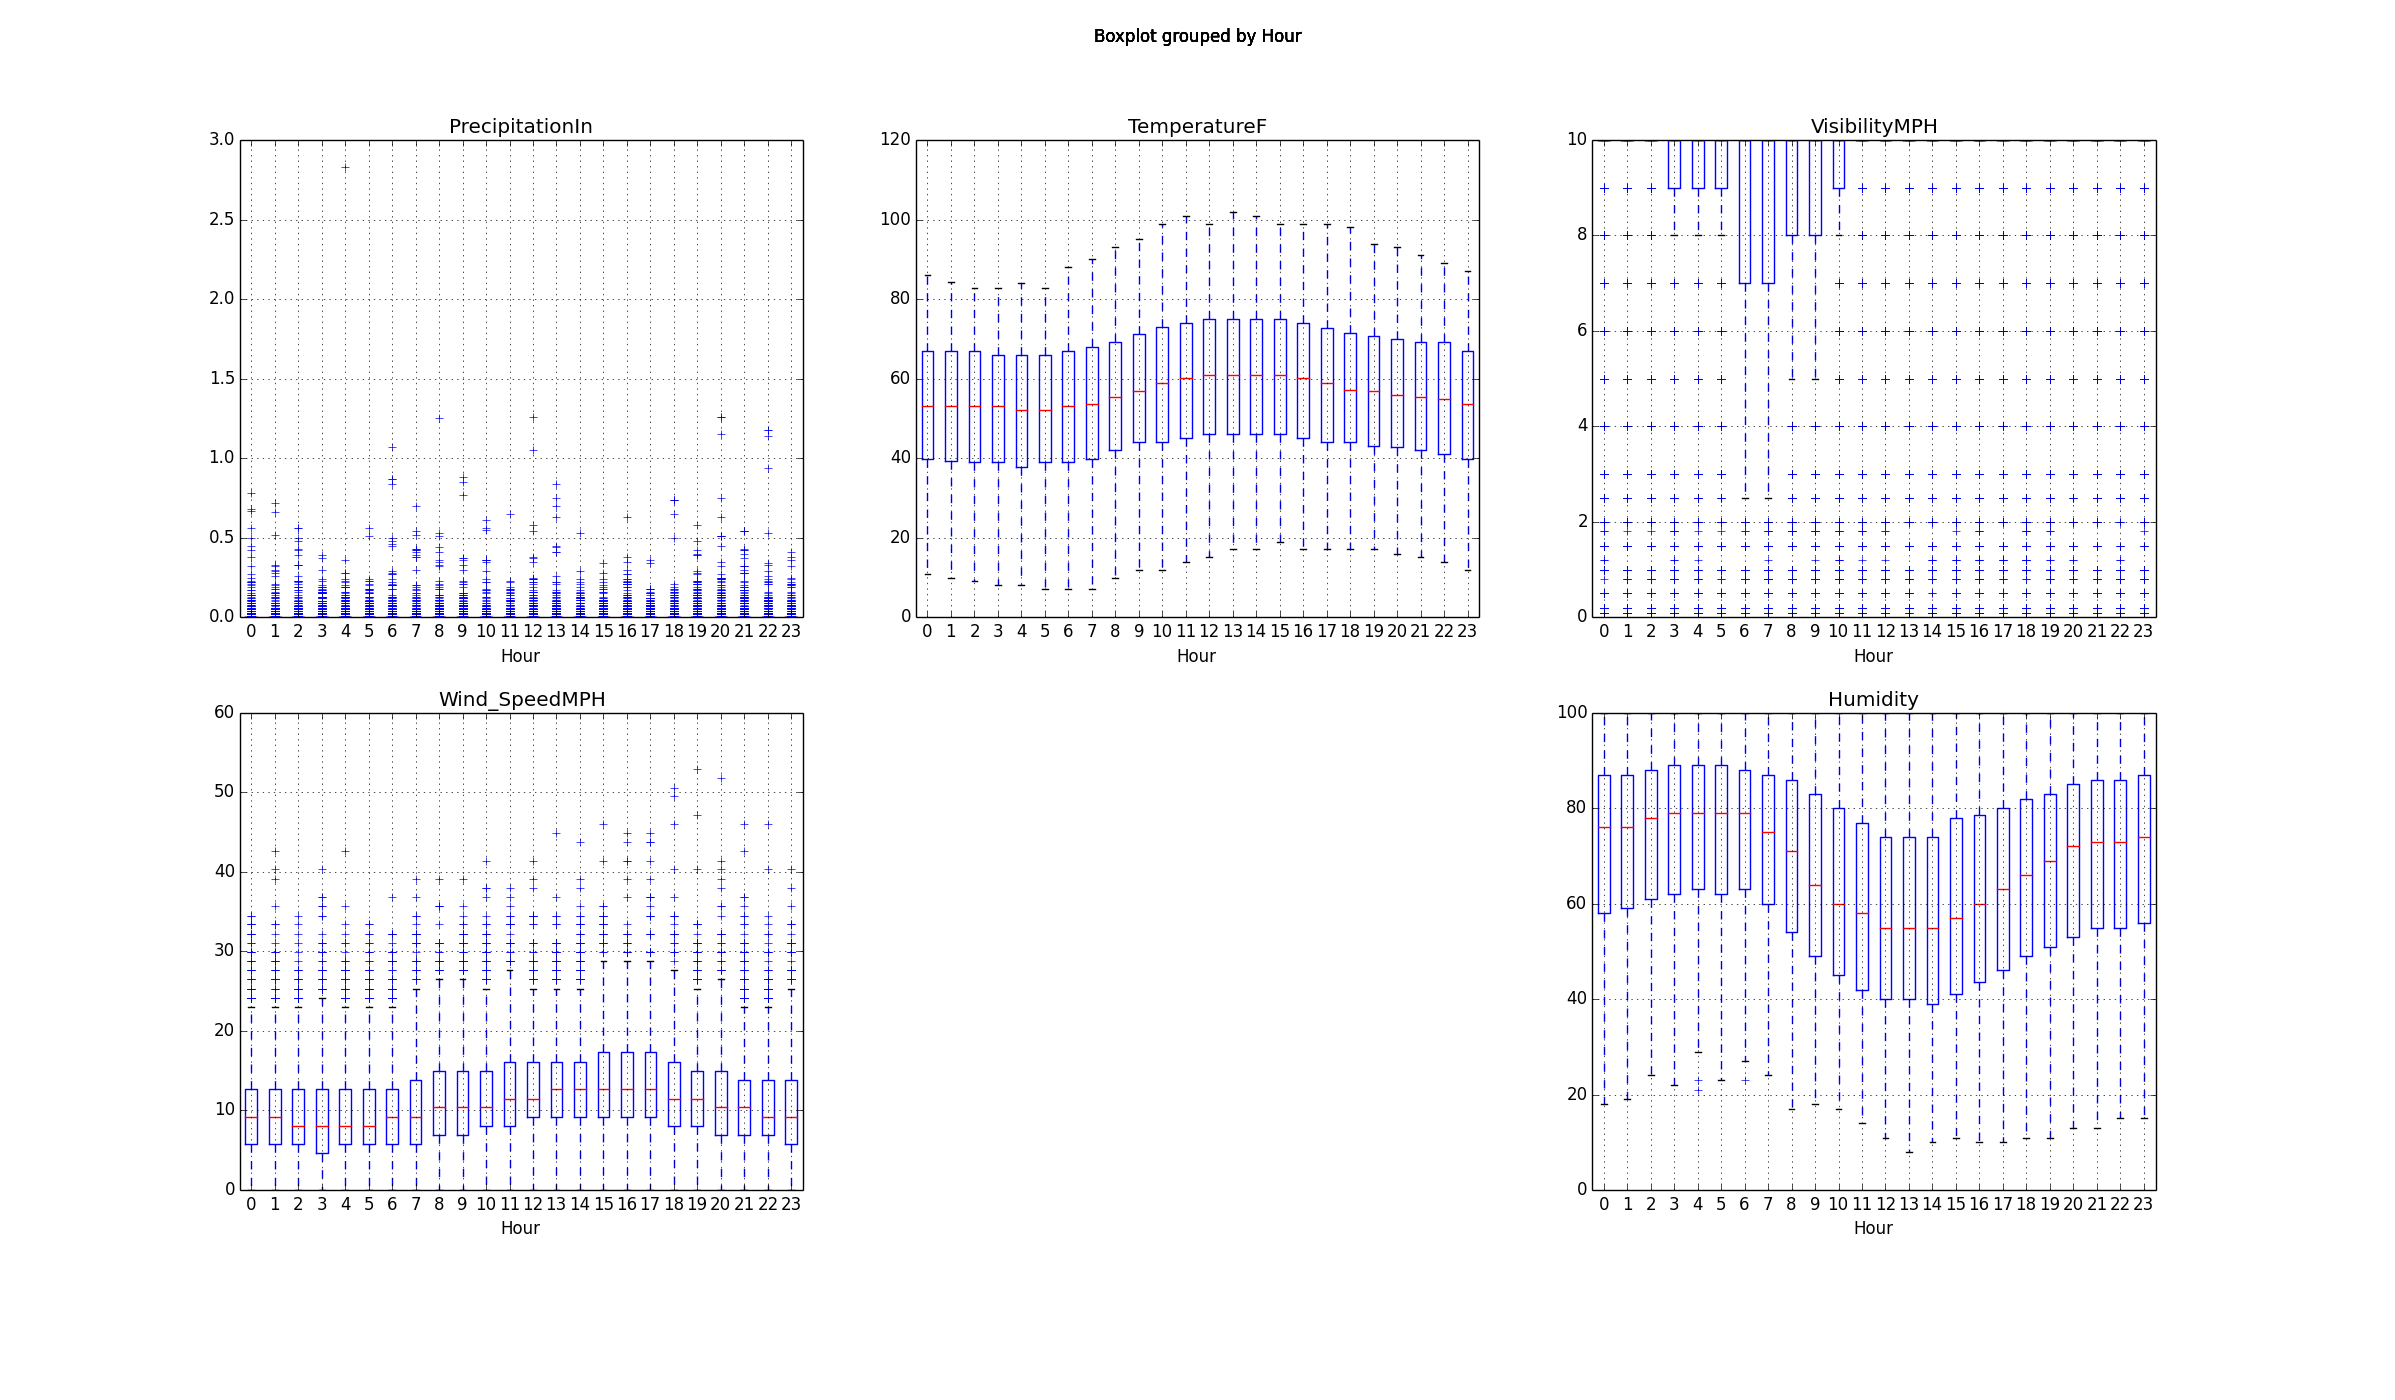
\includegraphics[scale=0.25]{./figures/boxplot_hourlyvariation.png}
\caption{Monthly variation in observations of weather variables}
\label{default}
\end{center}
\end{figure}

Variation over years of selected METAR weather variables every year.  

%%%concurrency table
\subsection*{Assessing Clusters}
When ground-truth labels are available, clusters can be assessed by various quantitative metrics that characterize the intra-cluster similarity of those labels versus the inter-cluster similarity of labels.  One example of such a metric is the RAND index, but there are various others.  More generally a ``confusion matrix" is a standard representation in Machine Learning to present the accuracy of an algorithm that models a categorial variable.  Typically, a model that has been fit using a training data set is asked to forecast the categorical variable in a distinct test data set.  The rows of the confusion matrix represent the actual values of the categorical variable in the test data set while the columns represent the model output values of the categorical variable using the model inputs from the test data set.  Each cell in the matrix is a count showing how many times the model predicted label x (column) when the actual observation was was label y (row).

We propose a novel method to use categorical data as ``psuedo-labels" for each observation.  The data we use for these psuedo-labels are the observed ``Condition" data column of METAR data, a categorical value.  Each day (sample of our data-matrix) has 24 such values and we propose three types of concurrency tables which allow use to analyze the similarity within and between the clusters using the frequency of occurrence of those categorical values.
\subsection*{Concurrency Tables}
The Condition data within METAR data describe weather conditions at an airport using a categorical variable.  The data are not ground-truth labels in the sense that we would explicitly seek to build a model of this data or claim that the data adequately summarize airport weather data for air traffic flow management initiative planning.  However, it is worthwhile to compare the results of cluster analysis to the Condition data, to see if, for example, days with the Condition label of ``Thunderstorm'' appear in one cluster while days with the Condition label of ``Clear'' appear in another cluster.  To explore the relationship between the METAR Condition data and identified clusters, we created concurrency tables.  The idea is similar to that of the Confusion Matrix described above.  Each row in a concurrency table refers to a specific Condition label and each column to a specific cluster output by a clustering algorithm.  Each cell in a concurrency table contains a count of the number of times a day was assigned to a specific Condition label (row) according to observed METAR data and a specific cluster (column) according to the results of a specific form of cluster analysis.

%Using results from:
%/Users/ashah/NoBackup/code/nasa/results/JFKexpert_kmeans_5.csv

Day-Aggregrated counts:
\begin{tabular}{lrrrrr}
\toprule
{} &     1 &     2 &     3 &      4 &      5 \\
\midrule
Blowing Snow                  &   - &   - &   - &      2 &      2 \\
Clear                         &   490 &   548 &  1936 &   2651 &   2674 \\
Fog                           &     5 &   230 &   233 &    238 &    462 \\
Haze                          &    55 &   181 &   202 &    207 &    310 \\
Heavy Rain                    &    22 &    74 &    80 &    155 &    238 \\
Heavy Snow                    &   - &     4 &     4 &      6 &     24 \\
Heavy Thunderstorms and Rain  &    36 &    62 &    66 &     71 &     86 \\
Ice Pellets                   &   - &     3 &     3 &      5 &      6 \\
Light Drizzle                 &     9 &   144 &   170 &    191 &    458 \\
Light Freezing Drizzle        &   - &     7 &     7 &      7 &     45 \\
Light Freezing Rain           &   - &     4 &     4 &      4 &     36 \\
Light Ice Pellets             &   - &     3 &     4 &      4 &     24 \\
Light Rain                    &   347 &   874 &  1330 &   1867 &   2799 \\
Light Rain Showers            &   - &   - &   - &      1 &      1 \\
Light Snow                    &   - &   194 &   304 &    463 &    814 \\
Light Thunderstorms and Rain  &    70 &   100 &   123 &    128 &    146 \\
Light Thunderstorms and Snow  &   - &   - &   - &    - &      1 \\
Mist                          &   - &    12 &    12 &     12 &     27 \\
Mostly Cloudy                 &  3410 &  4483 &  8639 &  11069 &  11501 \\
Overcast                      &  1135 &  2319 &  4619 &   5825 &   7271 \\
Partly Cloudy                 &   950 &  1075 &  2924 &   4404 &   4455 \\
Patches of Fog                &   - &     4 &     4 &      4 &      5 \\
Rain                          &    40 &   150 &   184 &    264 &    481 \\
Scattered Clouds              &  2068 &  2448 &  4859 &   6562 &   6659 \\
Shallow Fog                   &     2 &     2 &     2 &      2 &      2 \\
Smoke                         &   - &   - &     1 &      1 &      1 \\
Snow                          &   - &    15 &    18 &     40 &     71 \\
Squalls                       &   - &   - &     1 &      1 &      1 \\
Thunderstorm                  &    47 &    51 &    62 &     67 &     68 \\
Thunderstorms and Rain        &    24 &    35 &    40 &     47 &     53 \\
Thunderstorms with Small Hail &   - &     1 &     1 &      1 &      1 \\
Unknown                       &     5 &     7 &    11 &     16 &     20 \\
\bottomrule
\end{tabular}


Day-Most frequent counts:
\begin{tabular}{lrrrrr}
\toprule
{} &     1 &     2 &     3 &     4 &     5 \\
\midrule
Clear                  &   117 &   117 &   655 &   899 &   899 \\
Fog                    &   - &    72 &    72 &    72 &   132 \\
Haze                   &   - &    10 &    10 &    10 &    33 \\
Heavy Rain             &   - &   - &   - &    25 &    25 \\
Light Drizzle          &   - &    20 &    20 &    20 &    54 \\
Light Freezing Drizzle &   - &   - &   - &   - &    23 \\
Light Rain             &    48 &   282 &   397 &   566 &  1112 \\
Light Snow             &   - &   147 &   196 &   262 &   551 \\
Mostly Cloudy          &  2616 &  3205 &  6215 &  7825 &  7903 \\
Overcast               &   453 &  1181 &  2337 &  2885 &  3837 \\
Partly Cloudy          &   334 &   358 &  1146 &  1837 &  1837 \\
Rain                   &   - &     9 &     9 &     9 &     9 \\
Scattered Clouds       &  1113 &  1186 &  2126 &  2828 &  2852 \\
Snow                   &   - &   - &   - &    12 &    22 \\
\bottomrule
\end{tabular}


Day-Least frequent counts:
\begin{tabular}{lrrrrr}
\toprule
{} &    1 &    2 &    3 &    4 &    5 \\
\midrule
Clear                        &   73 &   79 &  252 &  343 &  348 \\
Fog                          &  - &   12 &   12 &   13 &   17 \\
Haze                         &   11 &   22 &   35 &   38 &   48 \\
Heavy Rain                   &    4 &   22 &   25 &   35 &   60 \\
Heavy Snow                   &  - &    4 &    4 &    4 &    4 \\
Heavy Thunderstorms and Rain &    5 &    7 &    7 &    9 &   14 \\
Ice Pellets                  &  - &  - &  - &  - &    1 \\
Light Drizzle                &    1 &   14 &   23 &   30 &   66 \\
Light Freezing Drizzle       &  - &  - &  - &  - &    2 \\
Light Freezing Rain          &  - &  - &  - &  - &    1 \\
Light Ice Pellets            &  - &    1 &    2 &    2 &    7 \\
Light Rain                   &   50 &   76 &  150 &  205 &  220 \\
Light Rain Showers           &  - &  - &  - &    1 &    1 \\
Light Snow                   &  - &    3 &    6 &   26 &   27 \\
Light Thunderstorms and Rain &   18 &   22 &   28 &   30 &   30 \\
Light Thunderstorms and Snow &  - &  - &  - &  - &    1 \\
Mist                         &  - &   10 &   10 &   10 &   14 \\
Mostly Cloudy                &  141 &  158 &  366 &  508 &  534 \\
Overcast                     &   94 &  109 &  281 &  383 &  397 \\
Partly Cloudy                &  189 &  206 &  486 &  661 &  665 \\
Patches of Fog               &  - &  - &  - &  - &    1 \\
Rain                         &   15 &   29 &   40 &   60 &   90 \\
Scattered Clouds             &  178 &  198 &  603 &  752 &  769 \\
Shallow Fog                  &    2 &    2 &    2 &    2 &    2 \\
Smoke                        &  - &  - &    1 &    1 &    1 \\
Snow                         &  - &  - &  - &  - &    3 \\
Squalls                      &  - &  - &    1 &    1 &    1 \\
Thunderstorm                 &    3 &    5 &    5 &    5 &    5 \\
Thunderstorms and Rain       &   10 &   18 &   19 &   22 &   27 \\
Unknown                      &    1 &    2 &    4 &    4 &    6 \\
\bottomrule
\end{tabular}


Condition Concurrency Tables for airport:EWR

%Using results from:
%/Users/ashah/NoBackup/code/nasa/results/EWRexpert_kmeans_5.csv

Day-Aggregrated counts:
\begin{tabular}{lrrrrr}
\toprule
{} &     1 &     2 &     3 &     4 &      5 \\
\midrule
Blowing Snow                        &   - &   - &    10 &    10 &     10 \\
Clear                               &   516 &  1446 &  1514 &  1546 &   3176 \\
Fog                                 &   - &   - &    70 &   147 &    149 \\
Haze                                &    29 &    35 &   191 &   416 &    525 \\
Heavy Ice Pellets                   &   - &   - &   - &     1 &      1 \\
Heavy Rain                          &     5 &    20 &    90 &   242 &    284 \\
Heavy Snow                          &   - &     1 &    18 &    53 &     53 \\
Heavy Thunderstorms and Rain        &     3 &    15 &    31 &    56 &    128 \\
Ice Pellets                         &   - &   - &     3 &    12 &     12 \\
Light Drizzle                       &     4 &    25 &   158 &   618 &    656 \\
Light Freezing Drizzle              &   - &   - &     7 &    48 &     48 \\
Light Freezing Rain                 &   - &   - &    17 &    52 &     52 \\
Light Ice Pellets                   &     3 &     8 &    14 &    39 &     41 \\
Light Rain                          &   151 &   547 &  1217 &  2633 &   3438 \\
Light Rain Showers                  &   - &   - &   - &     1 &      1 \\
Light Snow                          &    45 &   143 &   434 &   834 &    881 \\
Light Thunderstorms and Ice Pellets &   - &   - &   - &     2 &      2 \\
Light Thunderstorms and Rain        &     3 &    32 &    54 &    88 &    199 \\
Mist                                &   - &   - &   - &     3 &      3 \\
Mostly Cloudy                       &  1634 &  4074 &  5015 &  5404 &  11420 \\
Overcast                            &   886 &  2021 &  3168 &  4695 &   7838 \\
Partly Cloudy                       &   551 &  1833 &  1947 &  1988 &   3679 \\
Rain                                &     4 &    60 &   182 &   492 &    560 \\
Scattered Clouds                    &   881 &  2537 &  2835 &  2932 &   5746 \\
Smoke                               &   - &   - &   - &   - &      1 \\
Snow                                &     6 &    11 &    41 &    91 &     91 \\
Thunderstorm                        &     5 &    27 &    44 &    47 &    121 \\
Thunderstorms and Rain              &     4 &    17 &    30 &    55 &     94 \\
Unknown                             &     4 &    12 &    14 &    15 &     17 \\
\bottomrule
\end{tabular}
Day-Most frequent counts:
\begin{tabular}{lrrrrr}
\toprule
{} &     1 &     2 &     3 &     4 &     5 \\
\midrule
Blowing Snow           &   - &   - &     9 &     9 &     9 \\
Clear                  &   225 &   613 &   613 &   613 &  1235 \\
Fog                    &   - &   - &    10 &    32 &    32 \\
Haze                   &     8 &     8 &    40 &   118 &   137 \\
Heavy Rain             &   - &   - &    15 &    15 &    15 \\
Heavy Snow             &   - &   - &   - &    17 &    17 \\
Light Drizzle          &   - &   - &    11 &   152 &   152 \\
Light Freezing Drizzle &   - &   - &   - &    25 &    25 \\
Light Freezing Rain    &   - &   - &    10 &    10 &    10 \\
Light Rain             &    17 &   146 &   485 &  1457 &  1594 \\
Light Snow             &    14 &    51 &   295 &   627 &   639 \\
Mostly Cloudy          &  1113 &  2869 &  3367 &  3437 &  7909 \\
Overcast               &   510 &   953 &  1627 &  2476 &  4220 \\
Partly Cloudy          &   199 &   670 &   670 &   670 &  1222 \\
Rain                   &   - &   - &   - &    44 &    44 \\
Scattered Clouds       &   362 &  1017 &  1083 &  1083 &  2154 \\
\bottomrule
\end{tabular}
Day-Least frequent counts:
\begin{tabular}{lrrrrr}
\toprule
{} &    1 &    2 &    3 &    4 &    5 \\
\midrule
Blowing Snow                 &  - &  - &    1 &    1 &    1 \\
Clear                        &   55 &  144 &  145 &  153 &  371 \\
Fog                          &  - &  - &    8 &   12 &   12 \\
Haze                         &    5 &    8 &   31 &   41 &   58 \\
Heavy Ice Pellets            &  - &  - &  - &    1 &    1 \\
Heavy Rain                   &    1 &    8 &   15 &   56 &   63 \\
Heavy Snow                   &  - &    1 &    2 &    3 &    3 \\
Heavy Thunderstorms and Rain &  - &  - &    1 &    4 &    7 \\
Light Drizzle                &    1 &    8 &   24 &   53 &   66 \\
Light Freezing Drizzle       &  - &  - &    1 &    2 &    2 \\
Light Ice Pellets            &  - &  - &    1 &    4 &    4 \\
Light Rain                   &   14 &   56 &   75 &  105 &  191 \\
Light Rain Showers           &  - &  - &  - &    1 &    1 \\
Light Snow                   &   12 &   28 &   46 &   55 &   61 \\
Light Thunderstorms and Rain &  - &    7 &   12 &   16 &   25 \\
Mist                         &  - &  - &  - &    1 &    1 \\
Mostly Cloudy                &   95 &  233 &  247 &  266 &  511 \\
Overcast                     &   98 &  191 &  204 &  253 &  519 \\
Partly Cloudy                &   96 &  272 &  290 &  299 &  614 \\
Rain                         &    2 &   13 &   28 &   68 &   90 \\
Scattered Clouds             &  126 &  246 &  283 &  302 &  686 \\
Smoke                        &  - &  - &  - &  - &    1 \\
Snow                         &  - &  - &    2 &    9 &    9 \\
Thunderstorm                 &  - &    3 &    4 &    5 &   17 \\
Thunderstorms and Rain       &    2 &    5 &   10 &   13 &   34 \\
Unknown                      &  - &    7 &    8 &    8 &   10 \\
\bottomrule
\end{tabular}
Condition Concurrency Tables for airport:LGA
%Using results from:/Users/ashah/NoBackup/code/nasa/results/LGAexpert_kmeans_5.csv

Day-Aggregrated counts:
\begin{tabular}{lrrrrr}
\toprule
{} &     1 &     2 &     3 &     4 &      5 \\
\midrule
Blowing Snow                  &   - &   - &   - &     1 &      1 \\
Clear                         &   605 &  2618 &  2630 &  3566 &   3618 \\
Drizzle                       &   - &   - &     1 &     1 &      1 \\
Fog                           &     5 &     5 &    17 &    19 &    173 \\
Haze                          &    40 &   133 &   183 &   193 &    327 \\
Heavy Rain                    &    19 &    65 &   226 &   276 &    354 \\
Heavy Snow                    &   - &   - &    21 &    21 &     26 \\
Heavy Thunderstorms and Rain  &     2 &    52 &    84 &    86 &     91 \\
Ice Pellets                   &   - &   - &   - &   - &      3 \\
Light Drizzle                 &    19 &    58 &   225 &   255 &    374 \\
Light Freezing Drizzle        &     3 &     3 &     8 &     8 &     25 \\
Light Freezing Rain           &     1 &     1 &    25 &    25 &     66 \\
Light Ice Pellets             &     3 &     9 &    19 &    20 &     21 \\
Light Rain                    &   176 &   956 &  2143 &  2565 &   3161 \\
Light Rain Showers            &   - &     1 &     1 &     1 &      1 \\
Light Snow                    &   115 &   172 &   577 &   703 &    955 \\
Light Thunderstorms and Rain  &     8 &    87 &   110 &   116 &    129 \\
Light Thunderstorms and Snow  &   - &   - &     2 &     2 &      2 \\
Mist                          &     3 &     3 &     3 &     3 &     26 \\
Mostly Cloudy                 &  1823 &  7653 &  7940 &  9819 &  10413 \\
Overcast                      &  1084 &  4695 &  5847 &  7214 &   8654 \\
Partly Cloudy                 &   632 &  2851 &  2883 &  4185 &   4262 \\
Rain                          &    14 &    91 &   418 &   483 &    622 \\
Scattered Clouds              &   964 &  4073 &  4131 &  5424 &   5623 \\
Snow                          &     6 &     6 &    54 &    71 &    106 \\
Thunderstorm                  &     6 &    72 &    73 &    75 &     78 \\
Thunderstorms and Ice Pellets &   - &   - &     1 &     1 &      1 \\
Thunderstorms and Rain        &     8 &    32 &    49 &    56 &     57 \\
Unknown                       &   - &     2 &     2 &     4 &      4 \\
\bottomrule
\end{tabular}

Day-Most frequent counts:
\begin{tabular}{lrrrrr}
\toprule
{} &     1 &     2 &     3 &     4 &     5 \\
\midrule
Clear               &   271 &  1253 &  1253 &  1653 &  1666 \\
Haze                &   - &   - &   - &   - &    34 \\
Light Drizzle       &   - &   - &    41 &    41 &    48 \\
Light Freezing Rain &   - &   - &    13 &    13 &    44 \\
Light Rain          &    27 &   190 &   947 &  1031 &  1297 \\
Light Snow          &    54 &    65 &   412 &   470 &   671 \\
Mostly Cloudy       &  1299 &  5344 &  5414 &  6465 &  6651 \\
Overcast            &   605 &  2839 &  3512 &  4318 &  5367 \\
Partly Cloudy       &   238 &  1010 &  1010 &  1655 &  1655 \\
Rain                &   - &     9 &    48 &    48 &    63 \\
Scattered Clouds    &   389 &  1395 &  1395 &  1885 &  1925 \\
\bottomrule
\end{tabular}

Day-Least frequent counts:
\begin{tabular}{lrrrrr}
\toprule
{} &    1 &    2 &    3 &    4 &    5 \\
\midrule
Blowing Snow                 &  - &  - &  - &    1 &    1 \\
Clear                        &   68 &  354 &  356 &  459 &  466 \\
Drizzle                      &  - &  - &    1 &    1 &    1 \\
Fog                          &    1 &    1 &    5 &    5 &    6 \\
Haze                         &    6 &   22 &   31 &   31 &   55 \\
Heavy Rain                   &    1 &   11 &   29 &   38 &   45 \\
Heavy Snow                   &  - &  - &    8 &    8 &    8 \\
Heavy Thunderstorms and Rain &  - &    4 &    6 &    7 &    8 \\
Light Drizzle                &    4 &   12 &   34 &   44 &   72 \\
Light Freezing Drizzle       &  - &  - &    1 &    1 &    4 \\
Light Freezing Rain          &    1 &    1 &    1 &    1 &    1 \\
Light Ice Pellets            &    1 &    2 &    3 &    4 &    5 \\
Light Rain                   &   19 &  152 &  187 &  244 &  254 \\
Light Rain Showers           &  - &    1 &    1 &    1 &    1 \\
Light Snow                   &   10 &   21 &   22 &   28 &   29 \\
Light Thunderstorms and Rain &    3 &   21 &   22 &   22 &   27 \\
Mist                         &    3 &    3 &    3 &    3 &   11 \\
Mostly Cloudy                &  107 &  309 &  329 &  441 &  454 \\
Overcast                     &   66 &  266 &  280 &  362 &  367 \\
Partly Cloudy                &  115 &  453 &  461 &  571 &  579 \\
Rain                         &    4 &   25 &   46 &   58 &   67 \\
Scattered Clouds             &  133 &  557 &  567 &  687 &  718 \\
Snow                         &  - &  - &    2 &    4 &    6 \\
Thunderstorm                 &    3 &   12 &   12 &   12 &   12 \\
Thunderstorms and Rain       &    4 &   12 &   21 &   21 &   21 \\
\bottomrule
\end{tabular}
\section*{Conclusion}
In conclusion,
\bibliographystyle{abbrv}
\bibliography{all}
\end{document} 